\documentclass{article}

\usepackage{graphicx}
\usepackage{tikz}
\usepackage{tikzsymbols}
\usetikzlibrary{calc,patterns,shapes.geometric}
\pagestyle{empty}
\usepackage[margin=0pt]{geometry}
\geometry{papersize={14in,12in}}

\def\centerarc[#1](#2)(#3:#4:#5){\draw[#1] ($(#2)+({#5*cos(#3)},{#5*sin(#3)})$) arc (#3:#4:#5);}

\begin{document}
	\begin{figure}
		\centering
		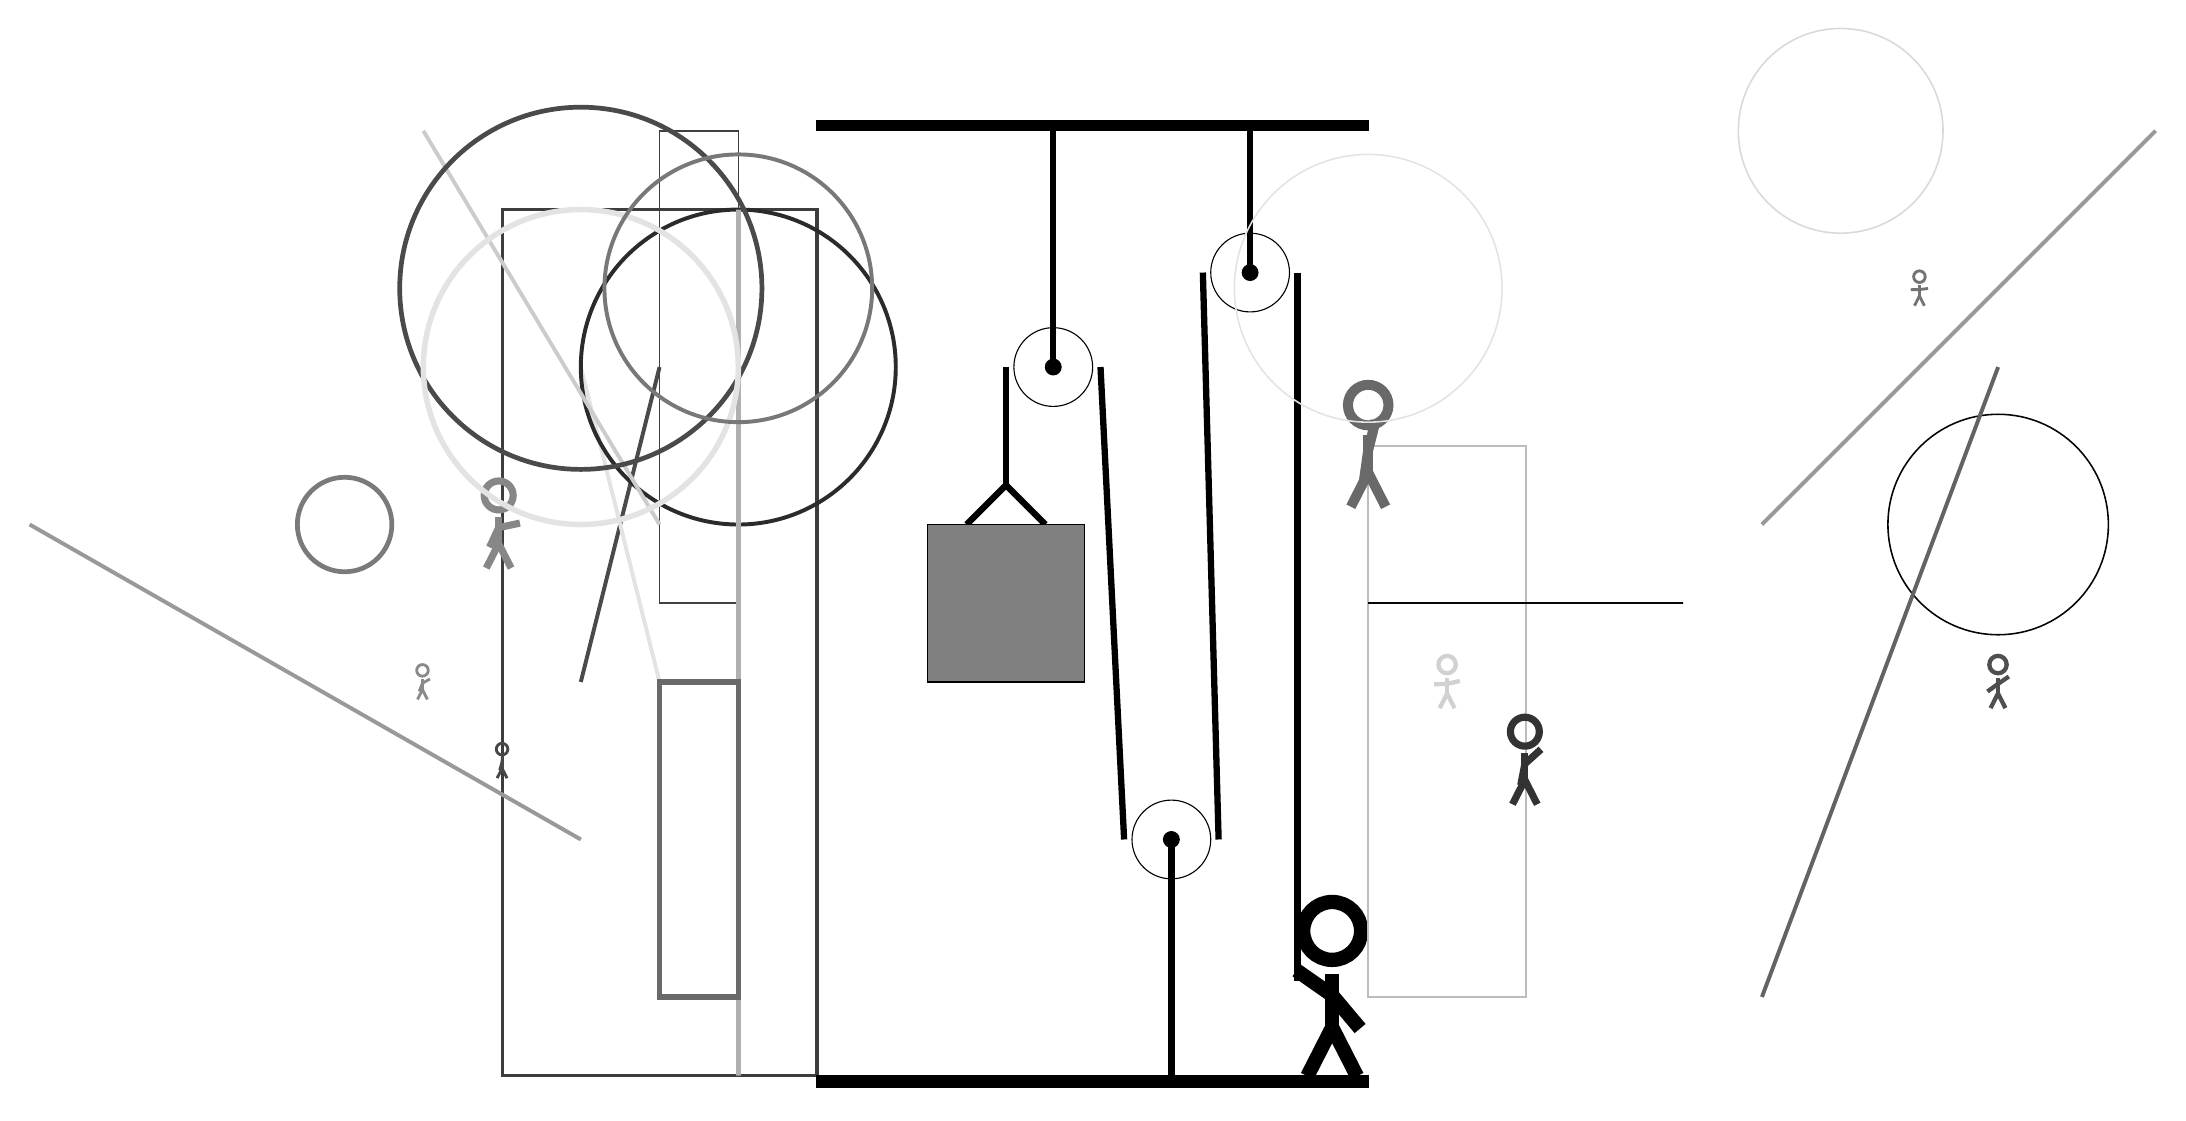
\begin{tikzpicture}
			%%%%% START %%%%%
			
			\draw[fill=black] (-2, 9) rectangle (5, 9.125);
			
			\draw (1, 6) circle (0.5);
			\draw[fill=black] (1, 6) circle (0.1);
			\draw[line width=0.8mm]  (1, 9) -- (1, 6);
			
			\draw[fill=white](2.5, 0) circle (0.5);
			\draw[fill=black] (2.5, 0) circle (0.1);
			\draw[line width=0.8mm]  (2.5, -3) -- (2.5, 0);
			
			\draw[fill=white](3.5, 7.2) circle (0.5);
			\draw[fill=black] (3.5, 7.2) circle (0.1);
			\draw[line width=0.8mm] (3.5, 9) -- (3.5, 7.2);
			
			\draw[line width=0.8mm] (-0.1, 4.0) -- (0.4, 4.5) -- (0.9, 4.0);
			\draw[fill=black!50] (-0.6, 4.0) rectangle (1.4, 2.0);
			
			\draw[line width=0.8mm] (0.4, 6) -- (0.4, 4.5);
			\centerarc[line width=0.8mm](1, 6)(0:180:0.6);
			\draw[line width=0.8mm](1.6, 6) -- (1.9, 0);
			\centerarc[line width=0.8mm](2.5, 0)(180:360:0.6);
			\draw[line width=0.8mm](3.1, 0) -- (2.9, 7.2);
			\centerarc[line width=0.8mm](3.5, 7.2)(0:180:0.6);
			\draw[line width=0.8mm](4.1, 7.2) -- (4.1, -1.8);
			
			\node at (4.5, -1.9) {\Strichmaxerl[10][-35][-50]};
			
			\draw[line width=0.2mm, color=black!26] (7, -2) rectangle (5, 5);
			
			\draw[line width=0.5mm, color=black!71](-5, 2) -- (-4, 6);
			\node[line width=0.5mm, color=black!69] at (13, 2) {\Strichmaxerl[3][36][34]};
			\draw[line width=0.5mm, color=black!40](10, 4) -- (15, 9);
			\draw[line width=0.5mm, color=black!11](-5, 6) -- (-4, 2);
			
			\node[line width=0.7mm, color=black!55] at (12, 7) {\Strichmaxerl[2][1][7]};
			\draw[line width=0.2mm, color=black!75] (-3, 9) rectangle (-4, 3);
			\node[line width=0.7mm, color=black!59] at (5, 5) {\Strichmaxerl[7][82][76]};
			\draw[line width=0.4mm, color=black!76] (-2, 8) rectangle (-6, -3);
			\draw [line width=0.6mm, color=black!52](-8, 4) circle (0.6);
			\node[line width=0.6mm, color=black!80] at (7, 1) {\Strichmaxerl[5][79][42]};
			\draw [line width=0.2mm, color=black!98](13, 4) circle (1.4);
			\node[line width=0.7mm, color=black!72] at (-6, 1) {\Strichmaxerl[2][74][87]};
			
			\draw [line width=0.5mm, color=black!83](-3, 6) circle (2.0);
			\node[line width=0.6mm, color=black!47] at (-6, 4) {\Strichmaxerl[5][65][12]};
			\draw[line width=0.5mm, color=black!61](10, -2) -- (13, 6);
			\draw[line width=0.5mm, color=black!20](-4, 4) -- (-7, 9);
			
			\draw[line width=0.7mm, color=black!31] (-3, -3) rectangle (-3, 8);
			\draw[line width=0.5mm, color=black!40](-5, 0) -- (-12, 4);
			\draw[line width=0.3mm, color=black!98] (5, 3) rectangle (9, 3);
			\draw [line width=0.2mm, color=black!11](5, 7) circle (1.7);
			
			\node[line width=0.3mm, color=black!46] at (-7, 2) {\Strichmaxerl[2][68][30]};
			\draw [line width=0.2mm, color=black!15](11, 9) circle (1.3);
			\draw[line width=0.7mm, color=black!59] (-4, -2) rectangle (-3, 2);
			\node[line width=0.5mm, color=black!18] at (6, 2) {\Strichmaxerl[3][2][13]};
			\draw [line width=0.6mm, color=black!71](-5, 7) circle (2.3);
			\draw [line width=0.4mm, color=black!69](-4, 2) circle (0.0);
			\draw [line width=0.7mm, color=black!11](-5, 6) circle (2.0);
			\draw[line width=0.4mm, color=black!96] (7, 2) rectangle (7, 2);
			
			\draw [line width=0.5mm, color=black!53](-3, 7) circle (1.7);
			
			\draw[fill=black] (-2, -3) rectangle (5, -3.15);
			
			%%%%% END %%%%%
		\end{tikzpicture}
	\end{figure}	
\end{document}